\subsection{Físico}

Estos se basan en la Capa de Tecnología. No se definen elementos de comportamiento físico separados.  Más bien, los elementos de comportamiento de la Capa de Tecnología (función de la tecnología, proceso, interacción, servicio y evento) se usan para modelar el comportamiento de todos los nodos, incluyendo el equipo físico. Dado que el equipo muy a menudo estará controlado por computadora o tendrá una estrecha relación con la tecnología de la información (piense también en los sensores, Internet de las cosas), su comportamiento puede describirse de manera integral utilizando los conceptos de comportamiento de la tecnología existente.

\newpage
\subsubsection{Elementos de la Estructura}

\begin{longtable}{|c| c| c|}
	\hline
	Concepto & Descripción & Representación \\ \hline
	Facilidad
	&
	\begin{tabular}{p{6cm}p{3cm}}
		Representa un recurso físico que tiene la capacidad de
		facilitar (por ejemplo, albergar o ubicar) el uso de equipos. Por lo general, se utiliza para modelar fábricas, edificios o construcciones al aire libre
	\end{tabular} 
	& 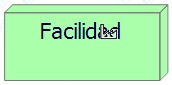
\includegraphics[width=0.1\linewidth, height=0.05\textheight]{imgs/conceptos/fisico/facilidad}
	\\
	\hline 
	Equipo
	& 
	\begin{tabular}{p{6cm}p{3cm}}
		El equipo comprende todos los elementos de procesamiento activos que llevan a cabo procesos físicos en los que se utilizan o transforman materiales.
	\end{tabular} 
	& 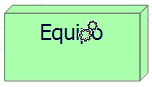
\includegraphics[width=0.1\linewidth, height=0.05\textheight]{imgs/conceptos/fisico/equipo}
	\\
	\hline
	Red de distribución
	&
	\begin{tabular}{p{6cm}p{3cm}} 
		Representa la distribución física o la infraestructura de transporte. Encarna la realización física de las rutas lógicas entre nodos. Una red de distribución conecta dos o más nodos. Una red de distribución puede realizar uno o más caminos.
	\end{tabular} 
	& 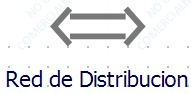
\includegraphics[width=0.1\linewidth, height=0.05\textheight]{imgs/conceptos/fisico/redDistribucion}
	\\
	\hline
	Material
	&
	\begin{tabular}{p{6cm}p{3cm}}  
		El material representa materia física tangible, con atributos como tamaño y peso. Suele utilizarse para modelar materias primas y productos físicos, y también fuentes de energía como el combustible.
	\end{tabular}
	& 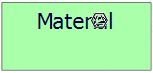
\includegraphics[width=0.1\linewidth, height=0.05\textheight]{imgs/conceptos/fisico/material}
	\\
	\hline
\end{longtable}